\documentclass{article}
\usepackage[dvipsnames]{xcolor} % for colorful text
\usepackage{tikz}             % for graphics
\usepackage{amsmath, amssymb} % for math symbols
\usepackage{hyperref}         % for creating links
\hypersetup{ colorlinks=true, linkcolor=blue}
\numberwithin{equation}{section}
\pagenumbering{roman}
\title{Thermal Physics}
\begin{document}

\maketitle
\tableofcontents
\pagebreak

\section{Boyle's Temperature}
At Boyle's temperature, $T_b$, $Z \to 1$\\
Using Van der Waals' equation,
$$P\left(1+\frac{a}{PV^2}\right) V\left(1-\frac{b}{V}\right) = RT$$
$$Z = \left(1+\frac{a}{PV^2}\right)^{-1} \left(1-\frac{b}{V}\right)^{-1}$$
$$Z = \left(1 - \frac{a}{PV^2}\right) \left(1+\frac{b}{V}\right)$$
$$Z = 1 + \frac{b}{V} - \frac{a}{PV^2} - \frac{ab}{PV^3}$$
$\because$ ab $\ll$ $V^3$,
at $T_B$, Z $\to$ 1,
$$\therefore \frac{b}{V} = \frac{a}{PV^2}$$
Using PV=RT,
$$b = \frac{a}{RT_b}$$
\begin{equation}
  \boxed{\textcolor{Mulberry}{T_b = \frac{a}{Rb}}} \label{eq:b1}
\end{equation}

\section{Critical Coefficients}
Using Van der waals' equation,
$$\left(P+\frac{a}{V^2}\right) \left(V-b\right) = RT$$
\begin{equation}
  P = \frac{RT}{\left(V-b\right)} - \frac{a}{V^2} \label{eq:c1}
\end{equation}
differentianting \eqref{eq:c1} w.r.t. V,
\begin{equation}
  \frac{dP}{dV} = - \frac{RT}{\left(V-b\right)^2} + \frac{2a}{V^3} \label{eq:c2}
\end{equation}
differentiating \eqref{eq:c2} w.r.t. V,
\begin{equation}
  \frac{d^2P}{dV^2} = \frac{2RT}{\left(V-b\right)^3} - \frac{6a}{V^4} \label{eq:c3}
\end{equation}
At the critical point,
$$\frac{dP}{dV} = 0  ,  \frac{d^2P}{dV^2} = 0$$
$\therefore$ \eqref{eq:c2} becomes,
\begin{equation}
  \frac{2a}{V_c^3} = \frac{RT_c}{\left(V_c-b\right)^2} \label{eq:c4}
\end{equation}
and \eqref{eq:c3} becomes,
\begin{equation}
  \frac{6a}{V_c^4} = \frac{2RT_c}{\left(V_c-b\right)^3} \label{eq:c5}
\end{equation}
Dividing \eqref{eq:c4} by \eqref{eq:c5},
$$\frac{V_c}{3} = \frac{\left(V_c-b\right)}{2}$$
$$2V_c = 3V_c - 3b$$
\subsection{Critical volume}
\begin{equation}
  \boxed{V_c = 3b} \label{eq:c6}
\end{equation}
Using \eqref{eq:c6} in \eqref{eq:c4},
$$\frac{2a}{27b^3} = \frac{RT_c}{4b^2}$$
\subsection{Critical temperature}
\begin{equation}
  \boxed{T_c = \frac{8a}{27Rb}} \label{eq:c7}
\end{equation}
Using \eqref{eq:c6} and \eqref{eq:c7} in \eqref{eq:c1},
$$P_c = \frac{4Ra}{27Rb^2} - \frac{a}{9b^2}$$
\subsection{Critical pressure}
\begin{equation}
  \boxed{P_c = \frac{a}{27b^2}} \label{eq:c8}
\end{equation}
\subsection{Critical compressibility factor}
$$Z = \frac{P_c V_c}{R T_c} = \frac{3}{8}$$
\subsection{Critical coefficient}
Critical coefficient is defined as the inverse of critical compressibility factor, i.e.,
$$K = \frac{1}{Z} = \frac{8}{3}$$

\section{Temperature of Inversion}
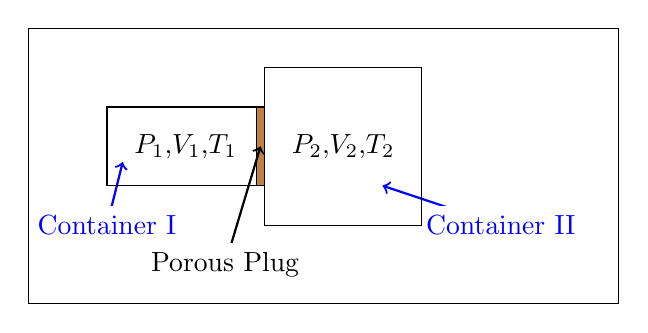
\begin{tikzpicture}
  % Outer Box
  \draw (-1,-2) rectangle (6.5,1.5);
  %Container 1
  \draw (1,0) node[align=center] {$P_1$,$V_1$,$T_1$};
  \draw[thick,->,blue] (0,-1) node[fill=white] {Container I} -- ((0.2,-0.2);
  \draw (0,-0.5) rectangle (2,0.5);
  %Porous Plug
  \filldraw[fill=brown] (1.9,-0.5) rectangle (2,0.5);
  \draw[thick,->] (1.5,-1.5) node[fill=white] {Porous Plug} -- (1.95,0);
  %Container 2
  \draw (3,0) node[align=center] {$P_2$,$V_2$,$T_2$};
  \draw[thick,->,blue] (5,-1) node[fill=white] {Container II} -- (3.5,-0.5);
  \draw (2,-1) rectangle (4,1);
\end{tikzpicture}
\\
When the temperature of incoming gas($T_1$) in Joule-Thompson effect is, then the temperature of the outcoming gas($T_2$) is,
\begin{itemize}
\item $T_2 > T_1$ when $T_1 > T_i$
\item $T_2 = T_1$ when $T_1 = T_i$
\item $T_2 < T_1$ when $T_1 < T_i$
\end{itemize}
Work done in overcoming intermolecular attractions,
\begin{align*}
  w &= \int_{V_1}^{V_2} P dV\\
  &= \int_{V_1}^{V_2} \frac{a}{V^2} dV\\
  &= - \frac{a}{V_2} + \frac{a}{V_1}
\end{align*}
Total work done by the gas,
$$W = (P_2 V_2 - P_1 V_1) + w$$
\begin{equation}
  W = (P_2 V_2 - P_1 V_1) + \left(\frac{a}{V_1} - \frac{a}{V_2}\right) \label{eq:i1}
\end{equation}
from Van der waals' equation, we know that
$$\left(P+\frac{a}{V^2}\right)(V-b) = RT$$
$$PV = RT + bP - \frac{a}{V} + \frac{ab}{V^2}$$
$$\because ab \ll V^2$$
\begin{equation}
  PV = RT + bP - \frac{a}{V} \label{eq:i2}
\end{equation}
Using \eqref{eq:i2} in \eqref{eq:i1},
$$W = RT + bP_2 - \frac{a}{V_2} - RT - bP_1 + \frac{a}{V_1} - \frac{a}{V_2} + \frac{a}{V_1}$$
\begin{equation}
  W = (P_2 - P_1)b + 2a \left(\frac{1}{V_1} - \frac{1}{V_2}\right) \label{eq:i3}
\end{equation}
Using $PV=RT$,
\begin{equation}
  V_1 = \frac{RT}{P_1} , V_2 = \frac{RT}{P_2} \label{eq:i4}
\end{equation}
Using \eqref{eq:i4} in \eqref{eq:i3},
$$W = (P_2 - P_1)b + \frac{2a}{RT}(P_1 - P_2)$$
$$W = (P_1 - P_2) \left[ \frac{2a}{RT} - b \right]$$
W = 0 when $T=T_i$\\
\[ \therefore \boxed{T_i = \frac{2a}{Rb}} \label{eq:i5} \tag{3.5} \]

\section{Relationship between $T_b$,$T_c$ and $T_i$}
Using \eqref{eq:b1}, \eqref{eq:c7} and \eqref{eq:i5},
$$T_c < T_b < T_i$$

\section{Maxwell's Relations}
From first law of thermodynamics,
\begin{equation}
  dU = TdS - PdV \label{eq:m1}
\end{equation}
we can write
$$T = \frac{\partial U}{\partial S} , P = -\frac{\partial U}{\partial T} $$
we can write U, S and V as functions of x and y where x and y are any of P, V, S or T,
\begin{equation}
  dU = \frac{\partial U}{\partial x}dx + \frac{\partial U}{\partial y}dy \label{eq:m2}
\end{equation}
\begin{equation}
  dS = \frac{\partial S}{\partial x}dx + \frac{\partial S}{\partial y}dy \label{eq:m3}
\end{equation}
\begin{equation}
  dV = \frac{\partial V}{\partial x}dx + \frac{\partial V}{\partial y}dy \label{eq:m4}
\end{equation}

using \eqref{eq:m2}, \eqref{eq:m3} and \eqref{eq:m4} in \eqref{eq:m1},
\begin{equation}
\frac{\partial U}{\partial x}dx + \frac{\partial U}{\partial y}dy = T\left[\frac{\partial S}{\partial x}dx + \frac{\partial S}{\partial y}dy \right] - P\left[\frac{\partial V}{\partial x}dx + \frac{\partial V}{\partial y}dy\right] \label{eq:m5}
\end{equation}

equating $dx$ terms of \eqref{eq:m5},
\begin{equation}
  \frac{\partial U}{\partial x} = T\frac{\partial S}{\partial x} - P\frac{\partial V}{\partial x} \label{eq:m6}
\end{equation}
differentiating \eqref{eq:m6} w.r.t. $y$,
\begin{equation}
  \frac{\partial^2 U}{\partial y \partial x} = \left(\frac{\partial T}{\partial y}\right)_x \left(\frac{\partial S}{\partial x}\right)_y + T\frac{\partial^2 S}{\partial y \partial x} - \left(\frac{\partial P}{\partial y}\right)_x \left(\frac{\partial V}{\partial x}\right)_y - P\frac{\partial^2 V}{\partial y \partial x} \label{eq:m7}
\end{equation}

equating $dy$ terms of \eqref{eq:m5},
\begin{equation}
  \frac{\partial U}{\partial y} = T\frac{\partial S}{\partial y} - P\frac{\partial V}{\partial y} \label{eq:m8}
\end{equation}
differentiating \eqref{eq:m8} w.r.t. $x$,
\begin{equation}
  \frac{\partial^2 U}{\partial x \partial y} = \left(\frac{\partial T}{\partial x}\right)_y \left(\frac{\partial S}{\partial y}\right)_x + T\frac{\partial^2 S}{\partial x \partial y} - \left(\frac{\partial P}{\partial x}\right)_y \left(\frac{\partial V}{\partial y}\right)_x - P\frac{\partial^2 V}{\partial x \partial y} \label{eq:m9}
\end{equation}

for a continuous function, F we have,
$$\frac{\partial^2 F}{\partial x \partial y}=\frac{\partial^2 F}{\partial y \partial x}$$
$\therefore$ from \eqref{eq:m7} and \eqref{eq:m9},
\begin{equation}
  \left(\frac{\partial T}{\partial y}\right)_x \left(\frac{\partial S}{\partial x}\right)_y - \left(\frac{\partial P}{\partial y}\right)_x \left(\frac{\partial V}{\partial x}\right)_y = \left(\frac{\partial T}{\partial x}\right)_y \left(\frac{\partial S}{\partial y}\right)_x - \left(\frac{\partial P}{\partial x}\right)_y \left(\frac{\partial V}{\partial y}\right)_x \label{eq:m10}
\end{equation}

\subsection{Equation I}
Using $x=P$ and $y=V$ in \eqref{eq:m10},
$$ \left(\frac{\partial T}{\partial V}\right)_P \left(\frac{\partial S}{\partial P}\right)_V - \left(\frac{\partial P}{\partial V}\right)_P \left(\frac{\partial V}{\partial P}\right)_V = \left(\frac{\partial T}{\partial P}\right)_V \left(\frac{\partial S}{\partial V}\right)_P - \left(\frac{\partial P}{\partial P}\right)_V \left(\frac{\partial V}{\partial V}\right)_P $$
$$\boxed{\left(\frac{\partial T}{\partial P}\right)_V \left(\frac{\partial S}{\partial V}\right)_P - \left(\frac{\partial T}{\partial V}\right)_P \left(\frac{\partial S}{\partial P}\right)_V = 1}$$

\subsection{Equation II}
Using $x=P$ and $y=S$ in \eqref{eq:m10},
$$ \left(\frac{\partial T}{\partial S}\right)_P \left(\frac{\partial S}{\partial P}\right)_S - \left(\frac{\partial P}{\partial S}\right)_P \left(\frac{\partial V}{\partial P}\right)_S = \left(\frac{\partial T}{\partial P}\right)_S \left(\frac{\partial S}{\partial S}\right)_P - \left(\frac{\partial P}{\partial P}\right)_S \left(\frac{\partial V}{\partial S}\right)_P$$
$$\boxed{\left(\frac{\partial T}{\partial P}\right)_S = \left(\frac{\partial V}{\partial S}\right)_P}$$

\subsection{Equation III}
Using $x=P$ and $y=T$ in \eqref{eq:m10},
$$\left(\frac{\partial T}{\partial T}\right)_P \left(\frac{\partial S}{\partial P}\right)_T - \left(\frac{\partial P}{\partial T}\right)_P \left(\frac{\partial V}{\partial P}\right)_T = \left(\frac{\partial T}{\partial P}\right)_T \left(\frac{\partial S}{\partial T}\right)_P - \left(\frac{\partial P}{\partial P}\right)_T \left(\frac{\partial V}{\partial T}\right)_P$$
$$\boxed{\left(\frac{\partial S}{\partial P}\right)_T = - \left(\frac{\partial V}{\partial T}\right)_P}$$

\subsection{Equation IV}
Using $x=V$ and $y=S$ in \eqref{eq:m10},
$$\left(\frac{\partial T}{\partial S}\right)_V \left(\frac{\partial S}{\partial V}\right)_S - \left(\frac{\partial P}{\partial S}\right)_V \left(\frac{\partial V}{\partial V}\right)_S = \left(\frac{\partial T}{\partial V}\right)_S \left(\frac{\partial S}{\partial S}\right)_V - \left(\frac{\partial P}{\partial V}\right)_S \left(\frac{\partial V}{\partial S}\right)_V$$
$$\boxed{\left(\frac{\partial P}{\partial S}\right)_V = - \left(\frac{\partial T}{\partial V}\right)_S}$$

\subsection{Equation V}
Using $x=V$ and $y=T$ in \eqref{eq:m10},
$$\left(\frac{\partial T}{\partial T}\right)_V \left(\frac{\partial S}{\partial V}\right)_T - \left(\frac{\partial P}{\partial T}\right)_V \left(\frac{\partial V}{\partial V}\right)_T = \left(\frac{\partial T}{\partial V}\right)_T \left(\frac{\partial S}{\partial T}\right)_V - \left(\frac{\partial P}{\partial V}\right)_T \left(\frac{\partial V}{\partial T}\right)_V$$
$$\boxed{\left(\frac{\partial S}{\partial V}\right)_T = \left(\frac{\partial P}{\partial T}\right)_V}$$

\subsection{Equation VI}
Using $x=S$ and $y=T$ in \eqref{eq:m10},
$$\left(\frac{\partial T}{\partial T}\right)_S \left(\frac{\partial S}{\partial S}\right)_T - \left(\frac{\partial P}{\partial T}\right)_S \left(\frac{\partial V}{\partial S}\right)_T = \left(\frac{\partial T}{\partial S}\right)_T \left(\frac{\partial S}{\partial T}\right)_S - \left(\frac{\partial P}{\partial S}\right)_T \left(\frac{\partial V}{\partial T}\right)_S$$
$$\boxed{\left(\frac{\partial P}{\partial T}\right)_S \left(\frac{\partial V}{\partial S}\right)_T - \left(\frac{\partial P}{\partial S}\right)_T \left(\frac{\partial V}{\partial T}\right)_S = 1}$$

\section{Statistical Mechanics}
\subsection{Fundamental Postulates of Statistical Mechanics}
\begin{itemize}
\item Any gas under consideration may be considered to be composed of large number of molecules which are constantly in motion and behave like very small elastic spheres.
\item All the cells in phase space are of equal size.
\item All accessible microstates corresponding to possible macrostates are equally probable.
\item The equilibrium state of a gas corresponds to the macrostate of maximum probability.
\item The total number of molecules is constant.
\item The total energy of the system is constant.
\end{itemize}

\subsection{Types of particles}
\subsubsection{Maxwell-Boltzmann Statistics}
Used to describe identical, distinguishable particles.
\subsubsection{Fermi-Dirac Statistics}
Used to describe identical, non-distinguishable particles with half-integral spins, i.e., $\frac{1}{2}$,$\frac{3}{2}$,etc...\\
Examples include electron, positron.
\subsubsection{Bose-Einstein Statistics}
Used to describe identical, non-distinguishable particles with integral spins, i.e., 0,1,2,etc...\\
Examples include photon, W boson.

\section{Maxwell-Boltzmann Energy Distribution Law}
Suppose the particles are distributed among $k$ energy levels $E_1,E_2,\dots,E_i,\dots,E_k$. Let $n_1,n_2,\dots,n_i,\dots,n_k$ be the number of independent quantum states associated with the energy levels. According to the basic statistical postulates
\begin{equation}
  N = n_1 + n_2 + \dots + n_i + \dots + n_k = \sum_i n_i \label{eq:mb1}
\end{equation}
and since the force of interation between particles are negligible, we have
\begin{equation}
  U = n_1 E_1 + n_2 E_2 + \dots + n_i E_i + \dots + n_k E_k \label{eq:mb2}
\end{equation}
Taking differential of equation \eqref{eq:mb1} and \eqref{eq:mb2}, we have
\begin{equation}
  dN = \sum_i dn_i = 0 \label{eq:mb3}
\end{equation}
and
\begin{equation}
  dU = \sum_i E_i dn_i = 0 \label{eq:mb4}
\end{equation}
\subsection{Maxwell-Boltzmann Statistical Count}
The number of ways of choosing $n_1$ particles for the first energy level($E_1$) is, thus, given by
$$x_1 = \frac{N!}{n_1!(N-n_1)!} = {}^NC_{n_1}$$
For the second state $E_2$, only $(N-n_1)$ particles are available and $n_2$ particles are in state $E_2$. The number of independent ways of choosing $n_2$ particles for the second energy level is
$$x_2 = \frac{(N-n_1)!}{n_2! (N-n_1-n_2)!} = {}^{N-n_1}C_{n_2}$$
Similarly for all energy levels. For the $k^{th}$ energy level we have
$$x_k = \frac{(N-n_1-n_2-\dots n_{k-1})!}{n_k! (N-n_1-n_2-\dots n_k)!} = {}^{(N-n_1-n_2-\dots n_{k-1})} C_{n_k}$$
Since these numbers are independent, the number of distinct ways of obtaining the distribution of particles among energy levels is given by
$$x = x_1 x_2 x_3 \dots x_i \dots x_k$$
\begin{equation}
  x = \frac{N!}{n_1! n_2! \dots n_k!} \label{eq:mb5}
\end{equation}
Now our next job is to find the number of independent ways in which the particles in the various energy level can be distributed among the quantum states in the respective levels. For example, in the energy level, containing $n_i$ particles, there are $g_i$ quantum states. Each of the $n_i$ particles can be in any one of the quantum states. Hence there are $g_i^{n_i}$ ways of arranging $n$ particles among $g_i$ quantum states available in the $i^{th}$ energy level.
$$W = \frac{N!}{n_1! n_2! \dots n_k!} \times g_1^{n_1} \times g_2^{n_2} \times \dots g_k^{n_k}$$
\begin{equation}
  W = N! \prod_{i=1}^{k} \left[\frac{g_i^{n_i}}{n_i!}\right] \label{eq:mb6}
\end{equation}
\subsection{Condition for most probable distribution}
The most probable distribution of the particles among the energy states in equilibrium is that for which the probability of occurence is maximum, i.e. for which \textbf{W is maximum}. For mathematical convenience, we consider the condition for maximum value of $\log W$. The condition for maximum value of $\log W$ is
\begin{equation}
  d(\log W) = 0 \label{eq:mb7}
\end{equation}
where W is a function of $n_1,n_2,\dots,n_k$.\\
Differentiating equation \eqref{eq:mb6}, we get
\begin{align*}
  d(\log W) &= \frac{\partial \log W}{\partial n_1}dn_1 + \frac{\partial \log W}{\partial n_2}dn_2 + \dots + \frac{\partial \log W}{\partial n_k}dn_k\\
  &= \sum_{i=1}^{k} \frac{\partial \log W}{\partial n_i}dn_i
\end{align*}
Applying the condition from equation \eqref{eq:mb7}, we get
\begin{equation}
  \sum_{i=1}^{k} \frac{\partial \log W}{\partial n_i}dn_i = 0 \label{eq:mb8}
\end{equation}
The solution of this equation is subject to the condition laid down by \eqref{eq:mb3} and \eqref{eq:mb4}. These conditions are introduced into equation \eqref{eq:mb8} by using the method of Lagrange's undetermined multipliers.\\
Let $\alpha$ and $\beta$ be these multipliers independent of $n_i$'s. We multiply \eqref{eq:mb3} by $-\alpha$ and \eqref{eq:mb4} by $-\beta$ and adding these equations to \eqref{eq:mb8}, we have
\begin{equation}
  \sum_{i=1}^{k}\left(\frac{\partial \log W}{\partial n_i} - \alpha - \beta E_i\right)dn_i \label{eq:mb9}
\end{equation}
\subsection{M-B Energy Distribution Law in General Form}
Taking logarithms of \eqref{eq:mb6}, we have
\begin{align*}
  \log W &= \log N! + \log \left[\prod_i \left(\frac{g_i^{n_i}}{n_i!}\right)\right]\\
  &= \log N! + \sum_{i=1}^{k} \left(n_i \log g_i - \log n_i!\right)
\end{align*}
Using sterlings formula, $\log x! = x(\log x - 1)$
\begin{equation}
  \log W = N \log N - N + \sum_{i=1}^{k}(n_i \log g_i - n_i \log n_i + n_i) \label{eq:mb10}
\end{equation}
Differentiating \eqref{eq:mb10} w.r.t. $n_i$,
$$\frac{d(\log W)}{dn_i} = \sum\left[\log g_i - \log n_i\right]\delta n_i$$
\begin{equation}
  \frac{d(\log W)}{dn_i} = \sum\left[-\log\left(\frac{n_i}{g_i}\right)\right]\label{eq:mb11}
\end{equation}
Substituting \eqref{eq:mb11} in \eqref{eq:mb9},
$$\sum\left[-\log\left(\frac{n_i}{g_i}\right) - \alpha - \beta E_i\right]\delta n_i = 0$$
$$\log\left(\frac{n_i}{g_i}\right) = -\alpha -\beta E_i$$
$$n_i = g_i e^{-\alpha-\beta E_i}$$
\begin{equation}
  n_i = g_i e^{-\alpha} e^{-\beta E_i} \label{eq:mb12}
\end{equation}
where $i=1,2,3,\dots k$\\
This equation is known as \textbf{Maxwell-Boltzmann energy distribution law} in the general form.\\
The value of $\beta$ is evaluated to be
$$\beta = \frac{1}{kT}$$
Substituting in \eqref{eq:mb12} we get
$$n_i = g_i e^{-\alpha} e^{-\frac{E_i}{kT}}$$
where $k$ is the Boltzmann  constant and T is the absolute temperature. The quantity $e^{-\frac{E_i}{kT}}$ is known as the \textbf{Boltzmann factor}.
From the fundamental postulates of statistical mechanics, we write,N, the total number of particles as
\begin{align*}
  N &= \sum_i n_i\\
  &= \sum_i g_i e^{-\alpha} e^{\frac{-E_i}{kT}}
\end{align*}
\begin{equation}
  e^{-\alpha} = \frac{N}{\sum_i g_i e^{\frac{-E_i}{kT}}} \label{eq:mb13}
\end{equation}
The quantity $\sum_i g_i e^{\frac{-E_i}{kT}}$ is the sum over all the states of the system and is called the \textbf{partition function} of the system denoted by Z. Thus
$$Z = \sum_i g_i e^{\frac{-E_i}{kT}}$$
Substituting in \eqref{eq:mb12}, we have
$$n_i = \frac{N}{Z} g_i e^{\frac{-E_i}{kT}}$$
\subsection{Maxwell-Boltzmann Speed Distribution Law}
The Maxwell-Boltzmann equation for distribution of energy among the molecules of an ideal gas is given by
$$n(E) dE = \frac{2\pi N}{(\pi kT)^{3/2}} E^{\frac{1}{2}} e^{\frac{-E}{kT}}dE$$

\end{document}
